
\chapter{Design}
\section{Analysis Review}



\section{Hardware Consumption}
Here will be discused wicht hardware is best sued for the task. The hardware will be evaluated by their
autonomy, the comunication protocol
\subsection{Autonomy}
As for the autonomy there are two main factors to consider, the batteries and the board consumption
\subsubsection{Batteries}
google sheets
\subsubsection{Board Consumption}



table

SIM7600 
table 6 and 34 (pg 20 and ) same voltage
2
SIM7020
peak 2A 20u in sleep mode 150mA

SIM7000 (GPS por NB-IoT e 2G fallback)
Consome: 11mA

SIM7080G - Nb-IoT
Quectel BG77

Quectel BG95-M3

 
GPS
MAX-M10S


IMU
BMI088 IMU Sensor
accelerometer 15uA  / and Gyroscope 2.7mA
ISM330BX
0.19mA / 0.6mA
BMI270


Unix Steptime

\subsection{Communication protocol}

table
EVKITST87M01-1 nb-iot
SIM7600 2g 3g 4g LTE CAT4

simbase chip availability

\begin{table}
    \centering
    \begin{tabular}{lllllll}
    Portugal & 2G & 3G & 4G & 5G & LTE & NB-IoT   \\
    Meo      & V  & V  & V  & -- & --  & --       \\
    Nos      & V  & V  & -- & -- & --  & --       \\
    Vodafone & V  & -- & V  & V  & V   & -- 
    \end{tabular}
\end{table}

europe coast
2g 4g


\subsection{Conclusion}
\section{Case Construction}
\section{Hardware Specification}
\subsection{SDCard}
\subsection{STM32}

STM32L010K4T6
microcontroler
ADC
UART
SPI
ONEWire
\subsection{BMI088 IMU Sensor}
gyroscope and acelerometer
\subsection{SIM7600E-H} 
The module SIM7600E-H, developed by SIMCom, is a 4G/3G/2G LTE module that comunicates via UART commads using an intern parser described on the module datasheet. 
The waveshare Board with the module, comes with a set of extra functionalities for extra support to the module normal usage.


The following image, taken from the Waveshare board datasheet, lists the hardware features.
\begin{figure}[H]%não estou gostando dessa foto
    \centering
    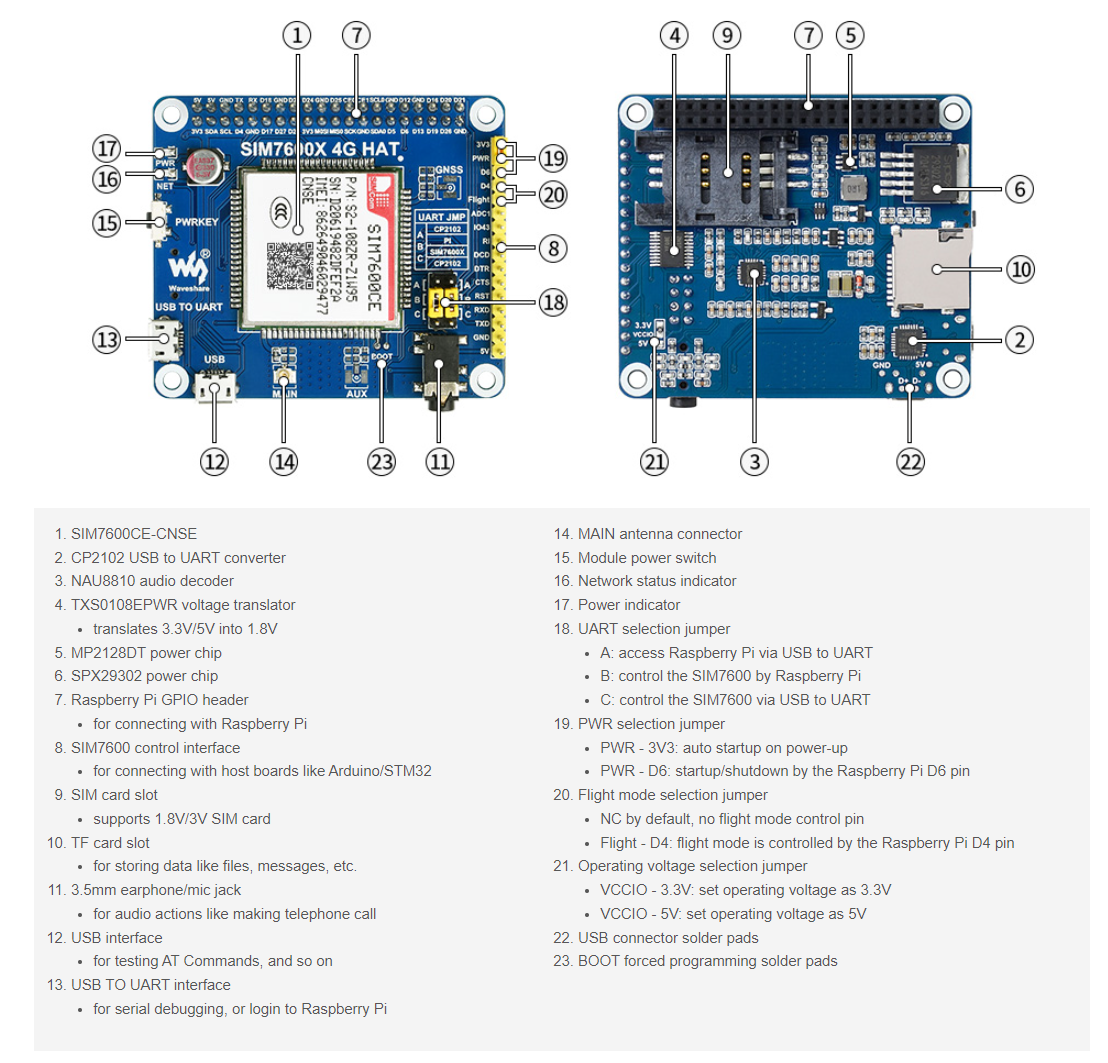
\includegraphics[width=1\textwidth]{images/chapter/design/SIM7600_board.png}
    \caption{SIM7600 datasheet}
    \label{fig:SIM7600 datasheet}
\end{figure}

The hardware configurations, as idicated on the datasheet should follow the leading steps.
%hw config

As for the UART communication, the list of commads are listed on the datasheet. 
As for better flow, here are listed the commadsused along the project and their functionalities. 
%commmand list

\subsection{Temperature}
DS18B20


\section{Tools and COTS}
\subsection{Tools}
\subsection{COTS}
\subsubsection{GPS and 4G module}
\subsubsection{Inkscape}
\subsubsection{draw.io}
\subsubsection{STM32 CUBEmx}
\subsubsection{\LaTeX}
\section{Software Specification}
\section{Theorical Concepts}